
% \section{Primer ap\'endice Comportamientos}
% Mostrar como est\'a implementada la arquitectura como software,
% 
% \section{Segundo ap\'endice Comportamientos}
% que habr\'ia que hacer para agregar un comportamiento nuevo, modificar
% uno existente.
% 
% \section{Tercer ap\'endice Comportamientos}
% Que hay que hacer para agregar un sensor o actuador nuevo.
% 
% \section{Quinto ap\'endice Comportamientos}
% Como es la interfaz con vision y porque se hizo de esa forma.

\section[Implementaci\'on del protocolo en PC]{Implementaci\'on del protocolo de comunicaci\'on del lado de la PC}
\subsection{Packet Server}
La implementaci\'on del protocolo en la PC la hicimos en C++, al igual que
el controlador y el m\'odulo de reconocimiento de basuras. Para la misma
implementamos los paquetes descriptos en el protocolo y un servidor de
env\'io y recepci\'on de los mismos a trav\'es del puerto serial. Tambi\'en
implementamos lo que llamamos handlers, quienes son los responsables de
convertir los comandos de la api del robot en paquetes y enviarlos al
servidor, as\'i como tambi\'en de recibir los paquetes de respuesta que
le incumben y proveerlos a la api de una forma que \'esta los entienda.
Mostramos el diagrama de \'esta relaci\'on en la figura
\ref{fig:diag_server_handler_packet}.
\\\indent
Como mencionamos anteriormente, hay un servidor que denominamos packet
server encargado del env\'io y recepci\'on de paquetes. El servidor s\'olo
se encarga de mandar una serie de bytes y de recibir los mismos, sin
inspeccionar de qu\'e tipo de paquete se trata. Provee
dos m\'etodos para realizar el env\'io y recepci\'on:
\begin{itemize}
	\item{sendPacket:} Su funci\'on es recibir un paquete y encolarlo para
		que el servidor lo env\'ie. Como el servidor es un thread diferente
		al de la api, no se interrumpe la recepci\'on o env\'io de paquetes.
	\item{registerHandler:} Registra un handler para un paquete enviado desde
		una placa con grupo $groupid$ e id de placa $boardid$. Cuando llega
		un paquete de dicha placa, el servidor invoca el m\'etodo
		handlePacket() del handler registrado.
\end{itemize}
La idea del m\'etodo handlePacket es que se limite s\'olo a guardar los
nuevos valores recibidos, ya que durante la invocaci\'on del mismo el
server no recibe ni env\'ia paquetes.
La clase packet provee funciones de utilidad para cualquier tipo de
paquete, tales como c\'alculo y verificaci\'on de CRC, seteo y obtenci\'on
de valores de los campos del paquete, entre otras.
\begin{figure}[ht]
	\centering
	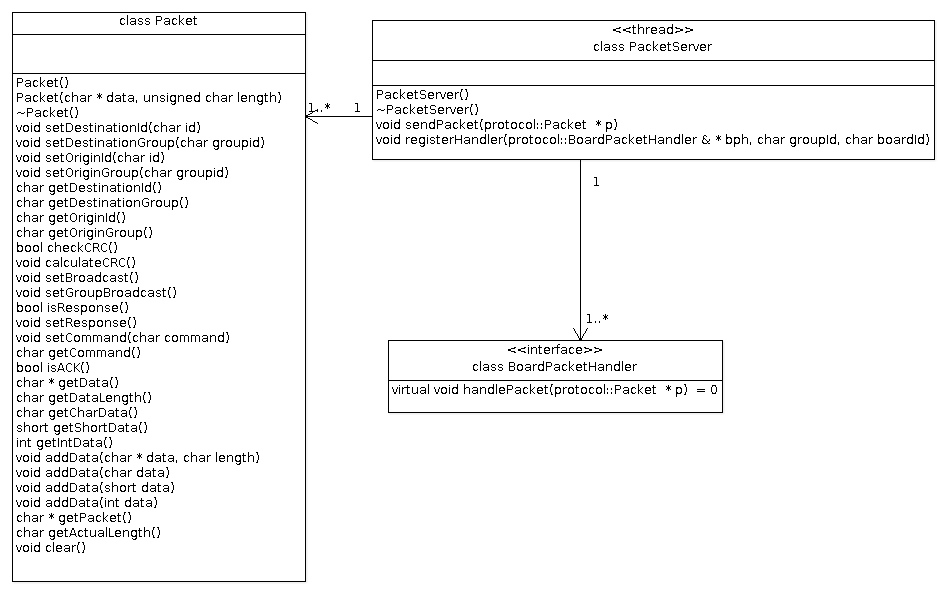
\includegraphics[scale=0.483]{comportamientos/figures/cs4.png}
	\caption[Diagrama de clases: Servidor de paquetes e interface]
			{Diagrama de clases. Estructura general del servidor de paquetes
			e interface para los handlers.}
	\label{fig:diag_server_handler_packet}
\end{figure}
\subsection{Packets}
Como indicamos en la figura \ref{fig:packet_group_board}, group packet extiende
a packet, agreg\'ando m\'etodos de utilidad para los comandos que todos
los grupos son capaces de recibir. Lo mismo sucede con board packet,
extendiendo de group packet ya que es m\'as espec\'ifico que este \'ultimo.

\begin{figure}[ht]
	\centering
	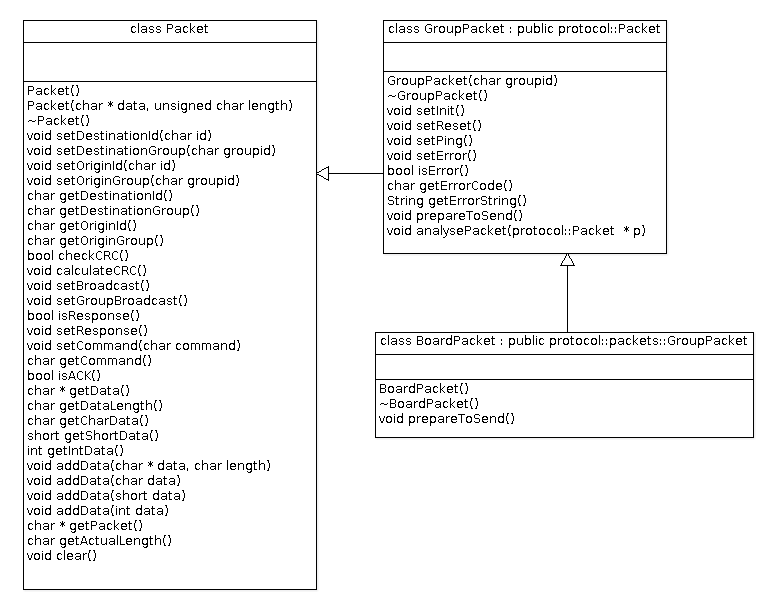
\includegraphics[scale=0.5]{comportamientos/figures/cs1.png}
	\caption[[Diagrama de clases: Estructura general]{Diagrama de clases. Estructura general de los paquetes.}
	\label{fig:packet_group_board}
\end{figure}

En las figuras \ref{fig:packet_specific_1} y \ref{fig:packet_specific_2}
mostramos los paquetes que extienden de board packet, espec\'ificos para
cada sensor o actuador que pueda haber en una placa. Como se puede observar,
cada paquete espec\'ifico tiene funciones que permiten obtener y setear
informaci\'on propia del sensor/actuador en cuesti\'on, respetando el
protocolo que propusimos.
\\\indent
Por ejemplo, BatteryPacket permite setear los thresholds o
umbrales a los cuales informar\'a que la bater\'ia se encuentra cargada o
en estado cr\'itico, respectivamente. Adem\'as permite obtener el valor
de carga de la bater\'ia.
\\\indent
A continuaci\'on damos un ejemplo de uso de un paquete. Supongamos que se
quiere saber la carga de la bater\'ia. Para \'esto instanciamos un
BatteryPacket con el id de grupo y placa correspondientes. El mismo se
encarga del seteo de los campos de grupo y placa de origen y destino,
tama\~no del paquete y comando. Le indicamos que queremos el valor de carga
con senseBattery(), que pone el comando correspondiente en el campo del
paquete. Una vez que tenemos el paquete armado, llamamos a la funci\'on
sendPacket() del packet server. Suponiendo que registramos un handler para
ese id de grupo y de placa, cuando el server reciba la respuesta de la placa
va a llamar al m\'etodo handlePacket() del handler. En la funci\'on,
instanciamos un BatteryPacket y llamamos a la funci\'on analysePacket()
con el paquete que recibimos. Finalmente, nos queda invocar al m\'etodo
getBatteryValue() de este paquete.

\begin{figure}[ht]
	\centering
	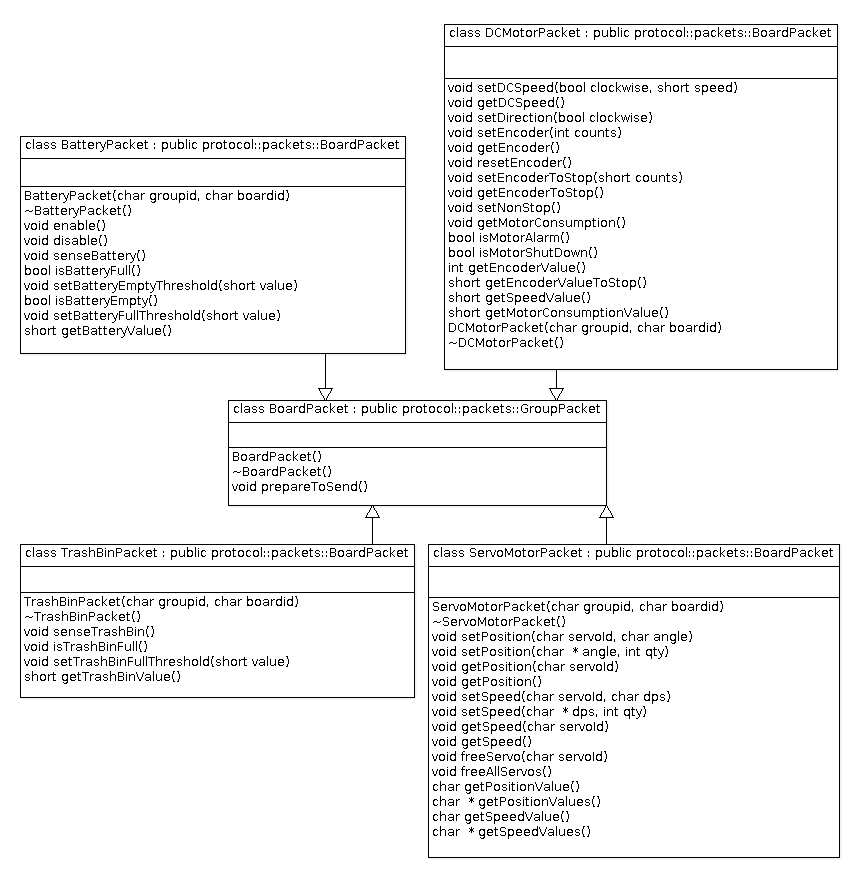
\includegraphics[scale=0.52]{comportamientos/figures/cs2.png}
	\caption[Diagrama de clases: Estructura paquetes 1]{Diagrama de clases. Estructura de los paquetes de motor, recipiente de basura, servos y bater\'ia.}
	\label{fig:packet_specific_1}
\end{figure}

\begin{figure}[ht]
	\centering
	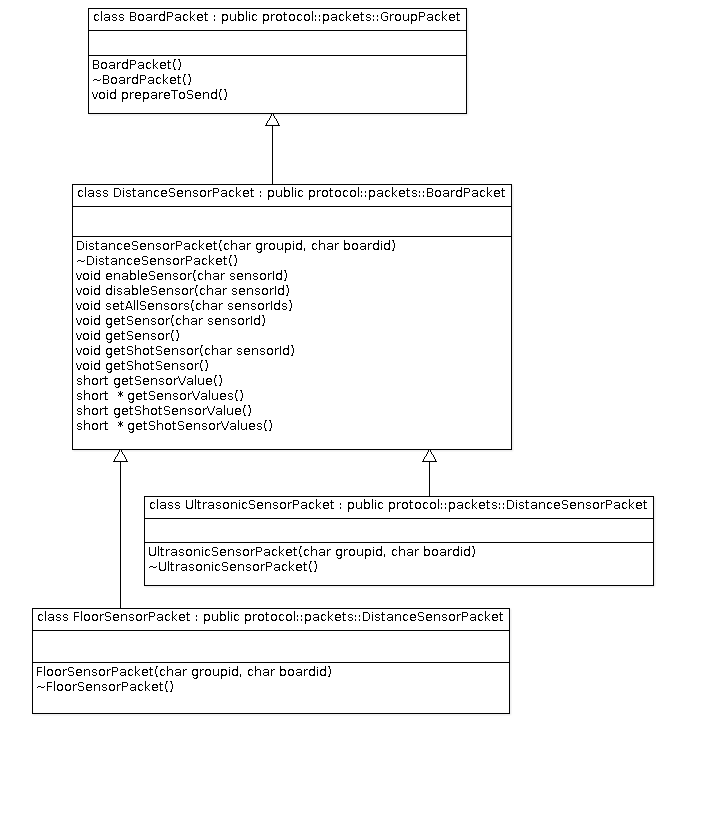
\includegraphics[scale=0.52]{comportamientos/figures/cs3.png}
	\caption[Diagrama de clases: Estructura paquetes 2]{Diagrama de clases. Estructura general de los paquetes para sensores de distancia.}
	\label{fig:packet_specific_2}
\end{figure}

\subsection{Handlers}
En las figuras \ref{fig:handler_specific_1} y \ref{fig:handler_specific_2}
mostramos los handlers implementados para que las implementaciones de los
sensores de la api del robot pudieran manejar los mismos, sin tener
conocimiento sobre el protocolo. Hay un handler por default,
DefaultBoardPacketHandler, para el caso en que no haya registrado un handler
para determinado id de grupo y placa. La funci\'on handlePacket del mismo
se encarga de imprimir por salida est\'andar cada campo del paquete en
formato hexadecimal.
\\\indent
Se puede observar que la cantidad de m\'etodos en los paquetes y en los
handlers no es la misma, y en algunos casos, hay m\'etodos que en el otro
no est\'an. \'Esto se debe a que los handlers son intermediarios entre
el protocolo y la api del controlador encargado de la ejecuci\'on de los
comportamientos. En algunos casos, el protocolo brinda m\'as opciones de
las que realmente utiliza el controlador para funcionar.
\begin{figure}[ht]
	\centering
	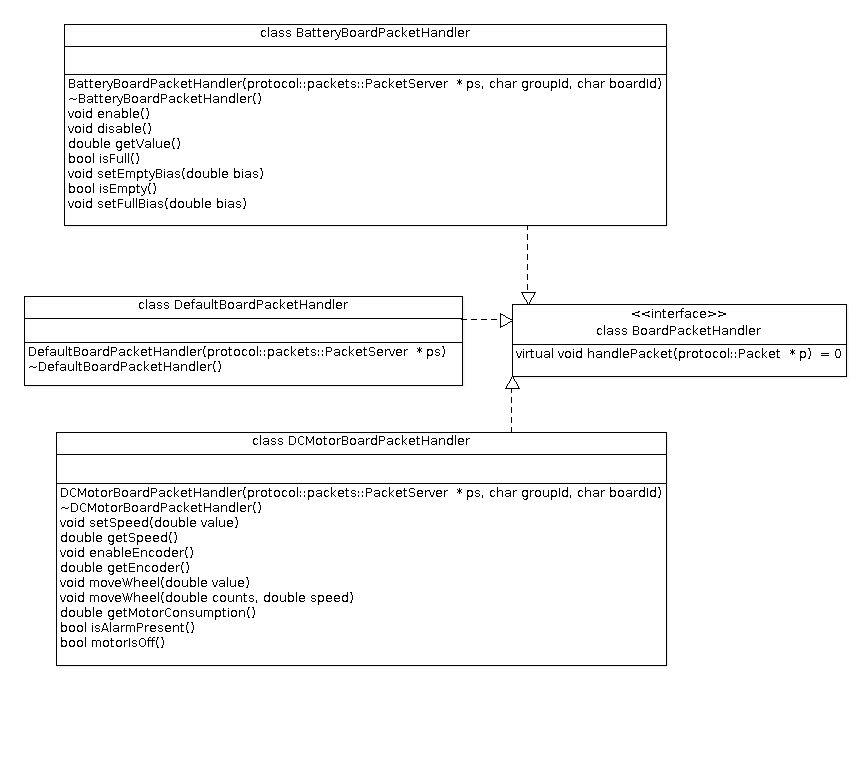
\includegraphics[scale=0.5]{comportamientos/figures/cs5.png}
	\caption[Diagrama de clases: Handlers 1]{Diagrama de clases. Handlers de paquetes default y para las placas de motor y 
	bater\'ia.}
	\label{fig:handler_specific_1}
\end{figure}

\begin{figure}[ht]
	\centering
	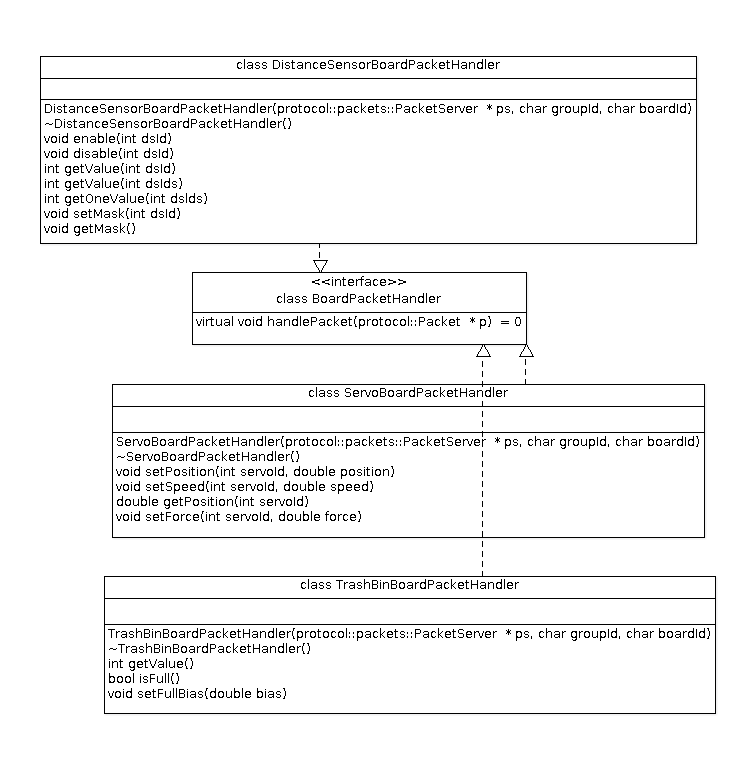
\includegraphics[scale=0.52]{comportamientos/figures/cs6.png}
	\caption[Diagrama de clases: Handlers 2]{Diagrama de clases. Handlers de paquetes para las placas de sensores de 
	distancia, servos y recipiente de residuos.}
	\label{fig:handler_specific_2}
\end{figure}


\begin{landscape}
\begin{figure}[h]
	\centering
	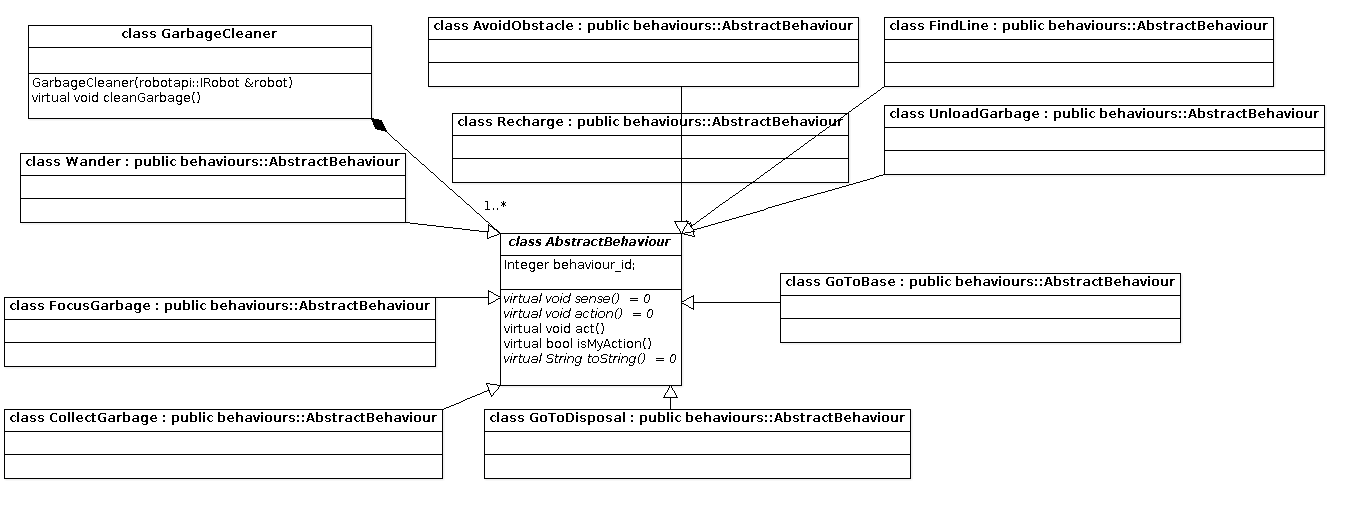
\includegraphics[scale=0.52]{comportamientos/figures/api1.png}
	\caption[Diagrama de clases: Handlers 2]{Diagrama de clases. Handlers de paquetes para las placas de sensores de 
	distancia, servos y recipiente de residuos.}
	\label{fig:diagclases}
\end{figure}
\end{landscape}
\begin{landscape}
\begin{figure}[h]
	\centering
	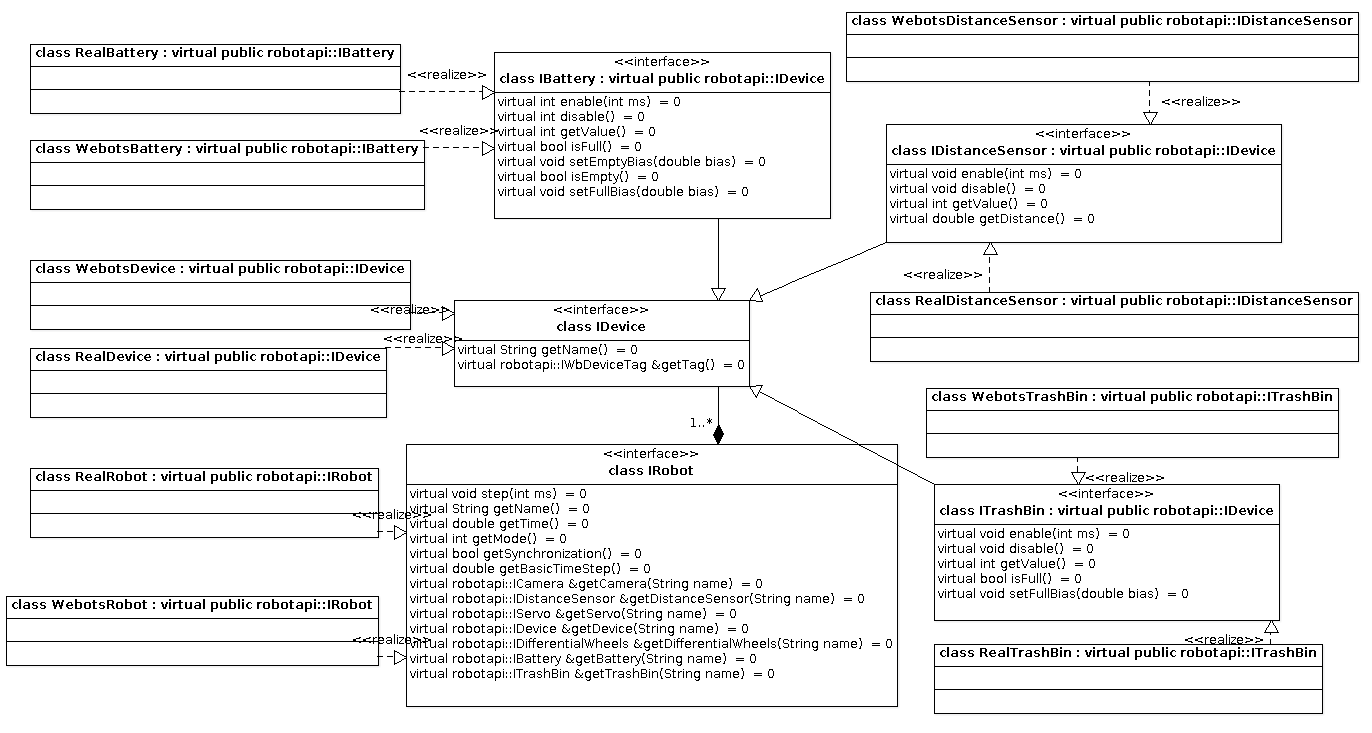
\includegraphics[scale=0.5]{comportamientos/figures/api2.png}
	\caption[Diagrama de clases: Handlers 2]{Diagrama de clases. Handlers de paquetes para las placas de sensores de 
	distancia, servos y recipiente de residuos.}
	\label{fig:diagclases}
\end{figure}
\end{landscape}


\subsection{Qu\'e hacer en caso que se modifique el protocolo}
En el caso que haya una modificaci\'on en el protocolo, se deber\'an
actualizar las clases afectadas por los cambios, y eventualmente,
los handlers correspondientes.
\\\indent
Supongamos el caso en el que se agrega un campo de 1 byte luego del tama\~no
total del paquete. \'Este cambio, en principio, s\'olo afecta la clase
Packet. En el caso que el campo indique algo sobre el grupo o placa,
tambi\'en afectar\'a a group packet o board packet, respectivamente.
En el caso que se ampl\'ie el set de comandos de un determinado sensor o
actuador, es necesario modificar el packet y handler asociados a los
mismos. Lo importante de \'esto es que los cambios est\'an localizados.
Es decir, un cambio en el protocolo llega como mucho hasta los handlers,
aislando a la api del controlador de posibles cambios.





